% Asset ID: FA21InequalitiesTikZ-004
% Source: FP1 PDF Ex 4C + teacher transcript
% Related lesson section: Section 9; Worked Example 12
% Purpose: Modulus graph for |x^2-19|<=5(x-1).
% Boundary status: Internal portal enrichment, not official CCEA Further Mathematics specification content.
\documentclass[tikz,border=8pt]{standalone}
\usepackage{amsmath}
\usepackage{xcolor}
\definecolor{Canvas}{HTML}{FAF9F6}
\definecolor{Ink}{HTML}{2C2C2E}
\definecolor{LineSoft}{HTML}{E5E5EA}
\definecolor{Gold}{HTML}{C5A059}
\definecolor{WarmPink}{HTML}{FBEFEF}
\begin{document}

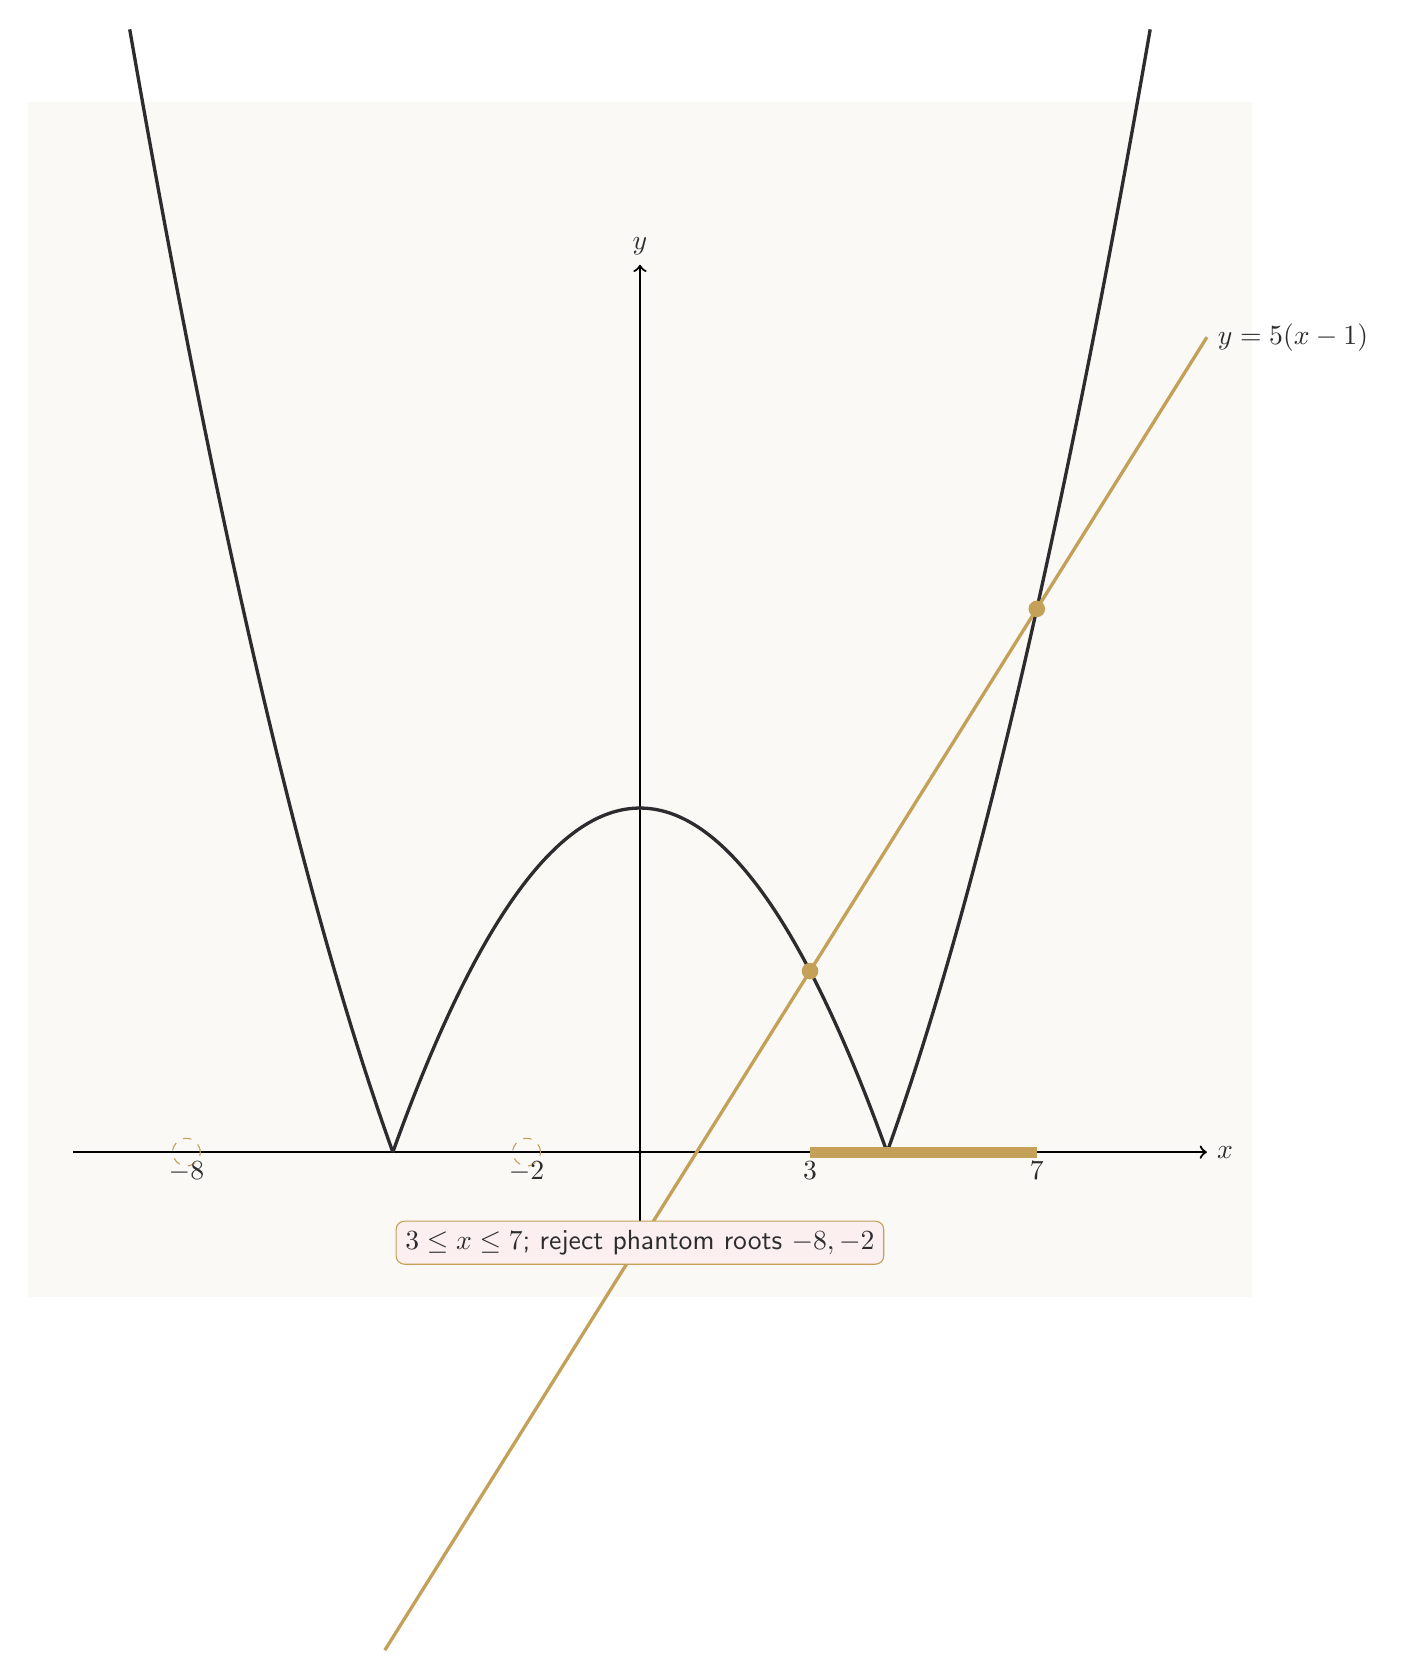
\begin{tikzpicture}[x=0.72cm,y=0.23cm,every node/.style={font=\sffamily,text=Ink}]
\fill[Canvas] (-10.8,-8) rectangle (10.8,58);
\draw[->,thick] (-10,0)--(10,0) node[right] {$x$};
\draw[->,thick] (0,-4)--(0,49) node[above] {$y$};
\draw[Ink,very thick,domain=-9:-4.36,samples=80,smooth] plot (\x,{\x*\x-19});
\draw[Ink,very thick,domain=-4.36:4.36,samples=120,smooth] plot (\x,{19-\x*\x});
\draw[Ink,very thick,domain=4.36:9,samples=80,smooth] plot (\x,{\x*\x-19});
\draw[Gold,very thick] (-4.5,-27.5)--(10,45) node[right] {$y=5(x-1)$};
\fill[Gold] (3,10) circle (3pt);\fill[Gold] (7,30) circle (3pt);
\draw[Gold,line width=4pt] (3,0)--(7,0);
\draw[Gold,dashed] (-8,0) circle (5pt);\draw[Gold,dashed] (-2,0) circle (5pt);
\node[below] at (-8,0) {$-8$};\node[below] at (-2,0) {$-2$};\node[below] at (3,0) {$3$};\node[below] at (7,0) {$7$};
\node[fill=WarmPink,draw=Gold,rounded corners=3pt] at (0,-5) {$3\le x\le7$; reject phantom roots $-8,-2$};
\end{tikzpicture}

\end{document}
